% To produce handouts, uncomment the following:
% \documentclass[handout]{beamer}
% \usepackage{pgfpages}
% \pgfpagesuselayout{2 on 1}[a4paper,border shrink=5mm]

\documentclass{beamer}

\usepackage[T1]{fontenc}
\usepackage{textcomp} 


\usepackage{futura}
\usetheme{Antibes}
\usecolortheme{beetle}
\xdefinecolor{myyellow}{rgb}{0.97, 0.90, 0.49}
\setbeamercolor{alerted text}{fg=myyellow}


\title{Categorization errors and differences in the quality of questions across countries}
\author{Daniel Oberski\\Willem Saris\\Jacques Hagenaars}
\institute
{
  \inst{}%
  Faculty of Social and Behavioural Sciences\\
  Tilburg University
  \and
  \inst{}%
  Survey Research Centre\\
  ESADE, Barcelona\\
  Universitat Ramon Llull\vspace{-1.2cm}
}
\date{}

\begin{document}

\begin{frame}
	\titlepage
	\begin{center}
	 
\includegraphics[width=4.5cm]{i/uvt.pdf}\hspace{.2cm}
	 
\includegraphics[width=2.8cm]{i/esade.pdf}	
  \end{center}	
\end{frame}

\section*{Outline}

%\begin{frame}
%\frametitle{Overview}
%	\tableofcontents
%\end{frame}

\section{Survey response model}

\begin{frame}
	\frametitle{The basic response model}
	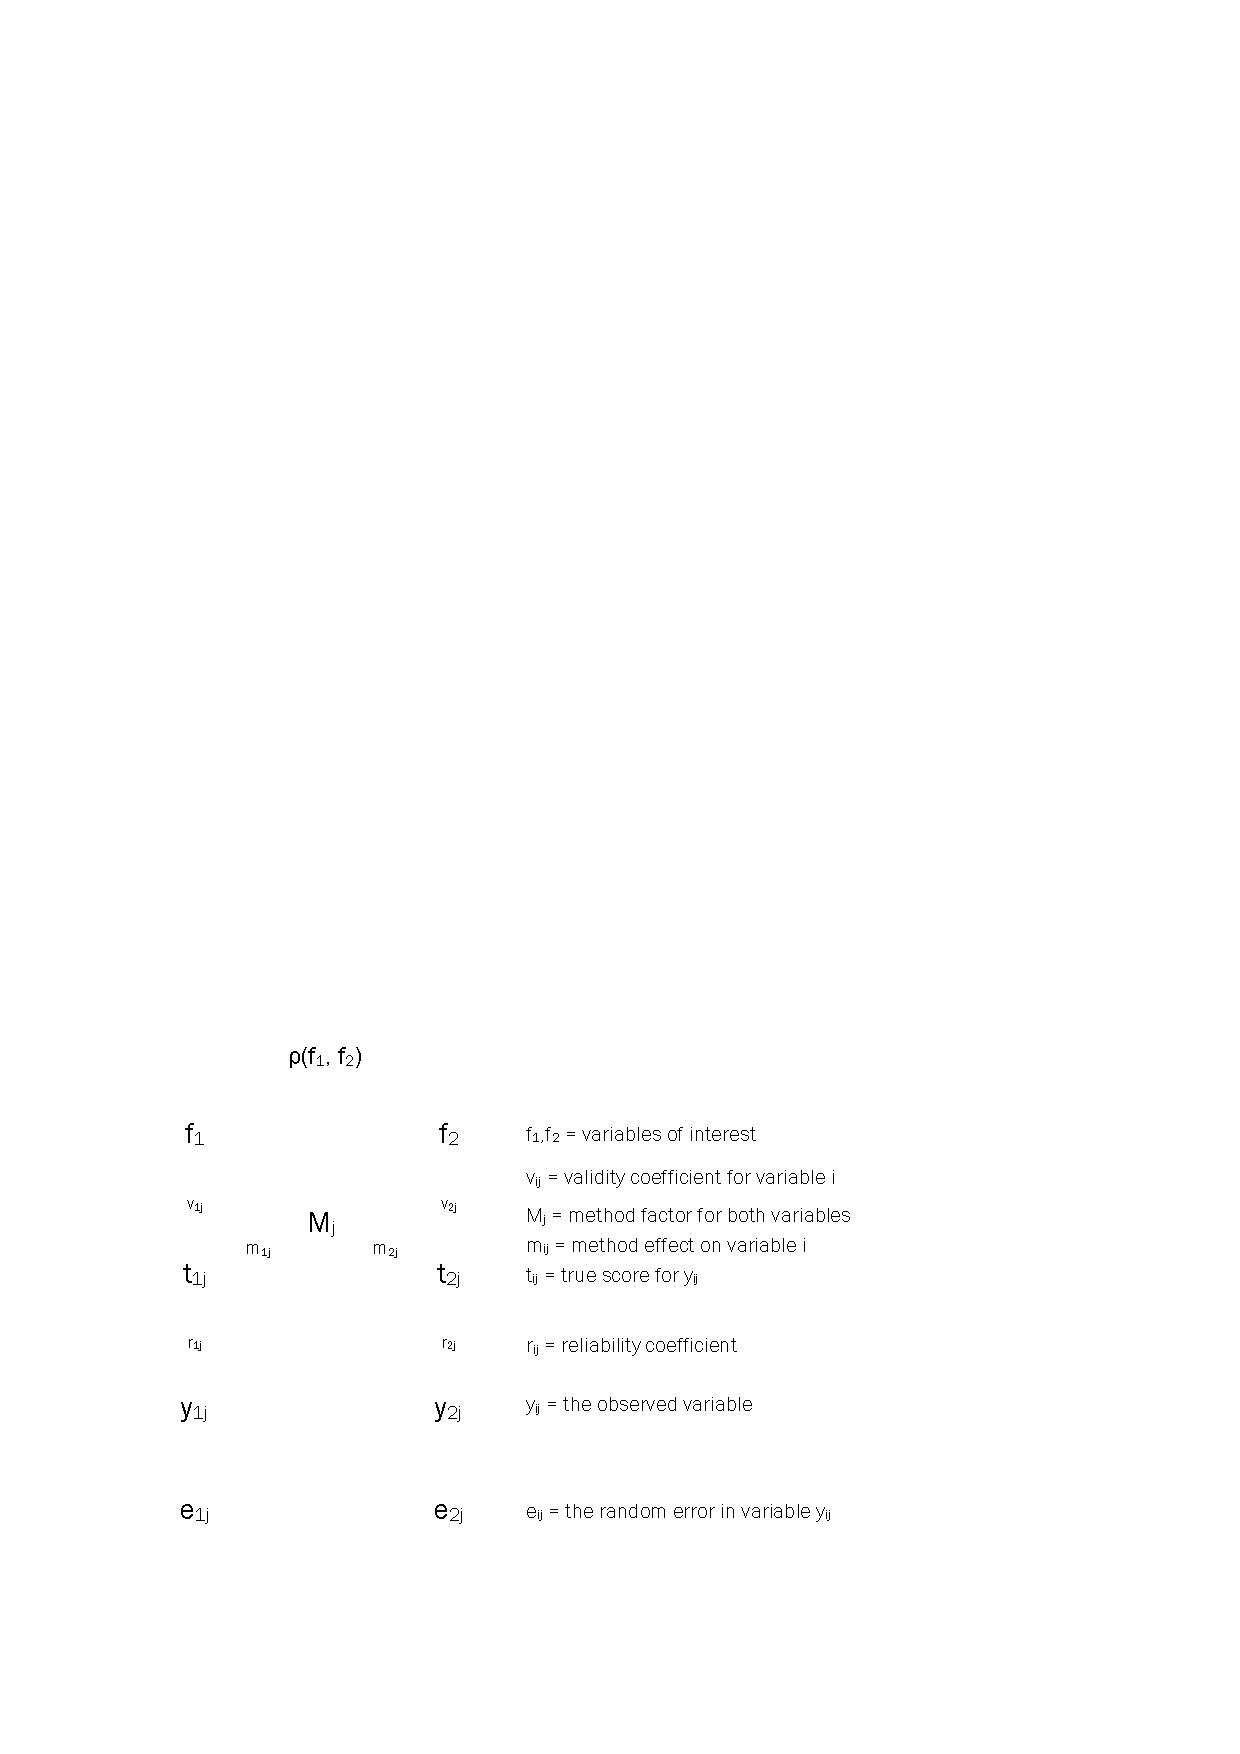
\includegraphics[height=7cm]{i/response-model.pdf}\\
\end{frame}

\begin{frame}
	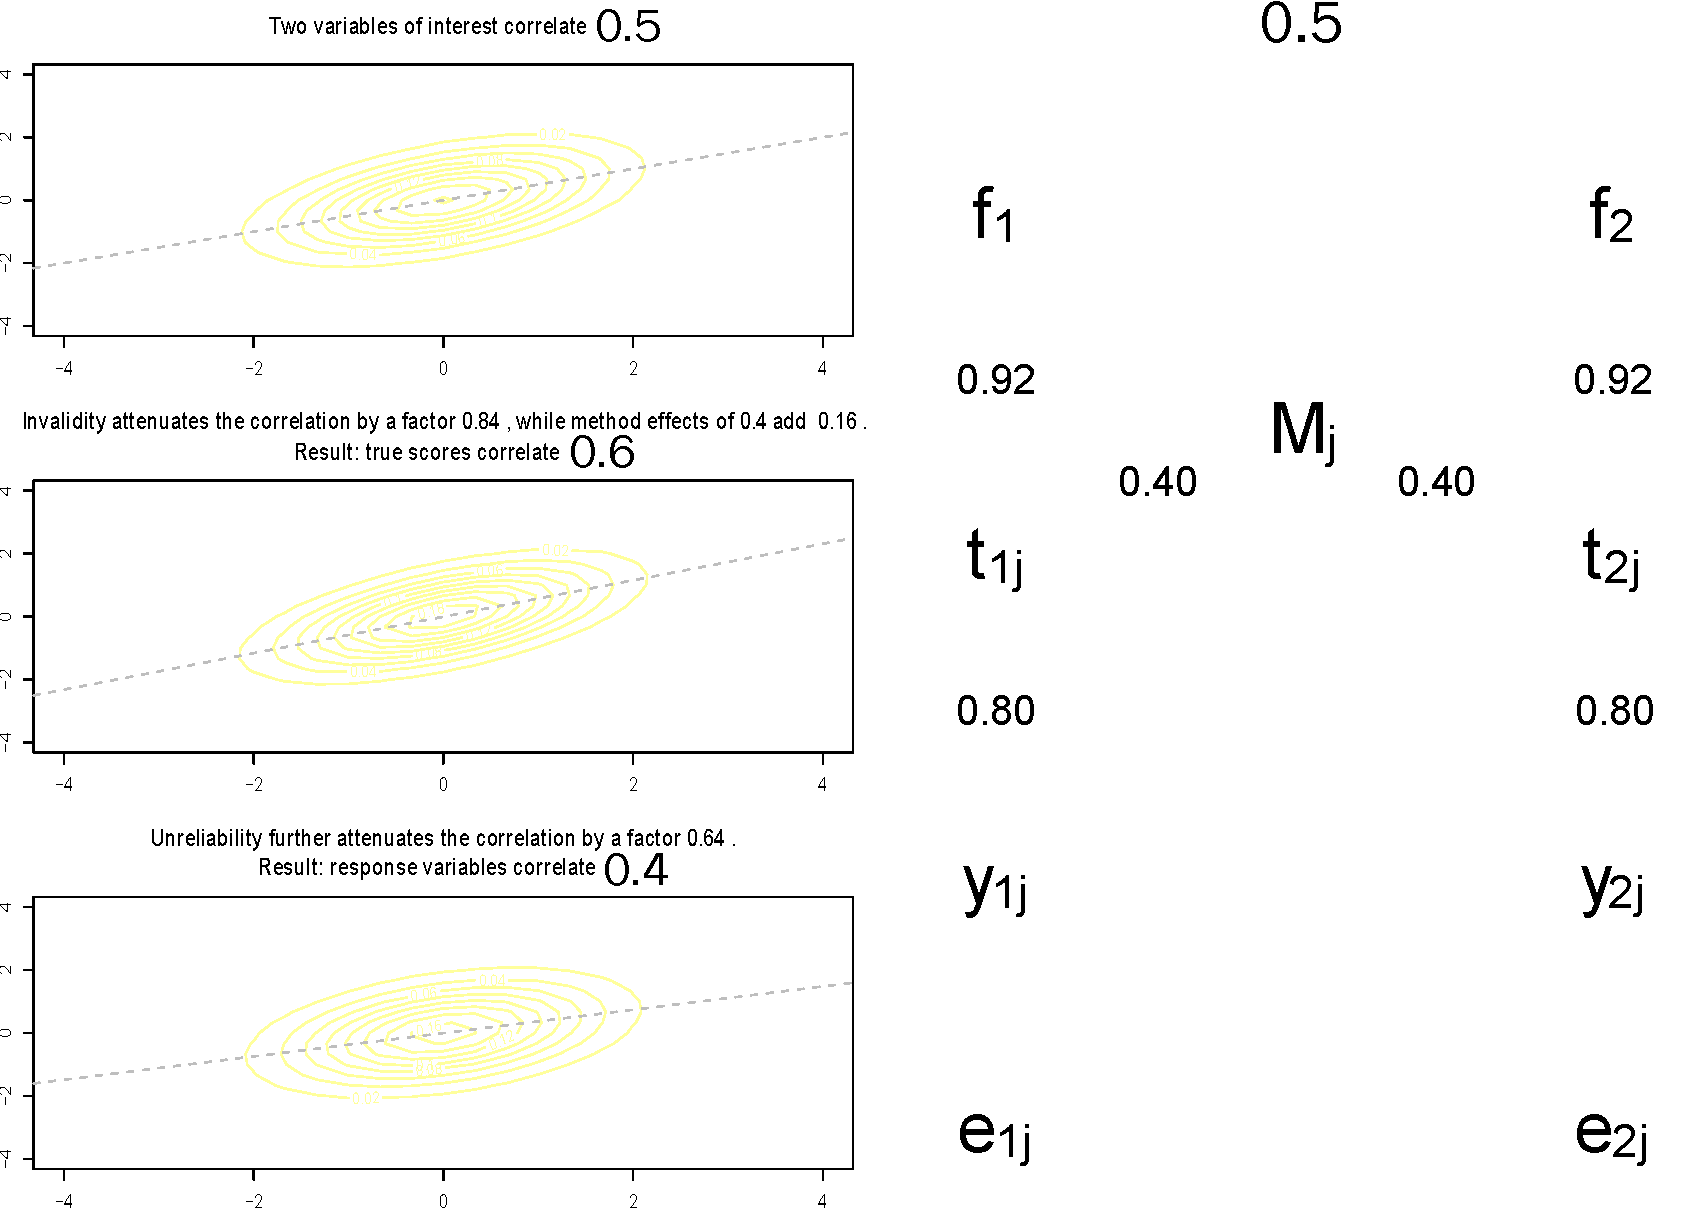
\includegraphics[width=\textwidth]{i/3_steps_together_CV.pdf}\\
\end{frame}


\begin{frame}	
	\frametitle{The basic response model}
	\begin{itemize}[<alert@+>]
		\item The quality coefficient $q$ is the product of the reliability and validity coefficients:
		\item $q = vr$
		\item The square $q^2$ is called the 'total quality' of a measure.
		\item It is the percentage of variance in the observed variable that can be explained by the latent variable of interest.
		\item The observed variables are assumed to be continuous.
	\end{itemize}
\end{frame}	

\begin{frame}
   \frametitle{The basic response model, revised}
   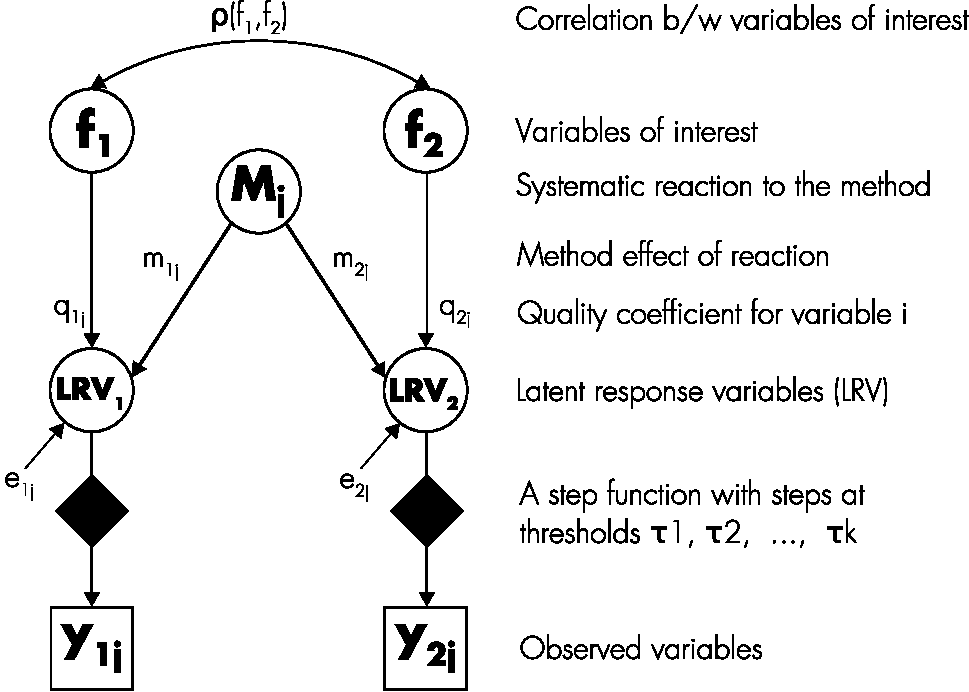
\includegraphics[height=7cm]{../latex/i/response_model_categorical.pdf}
\end{frame}


\begin{frame}
	\frametitle{Categorisation of continuous variables}

    Our model assumes that there are \emph{unobserved} continuous latent response variables (LRV) that have been categorised into the \emph{observed} categorical variables.

 \begin{columns}<2->[T]
 	\begin{column}{4.5cm} \textbf{country A}

	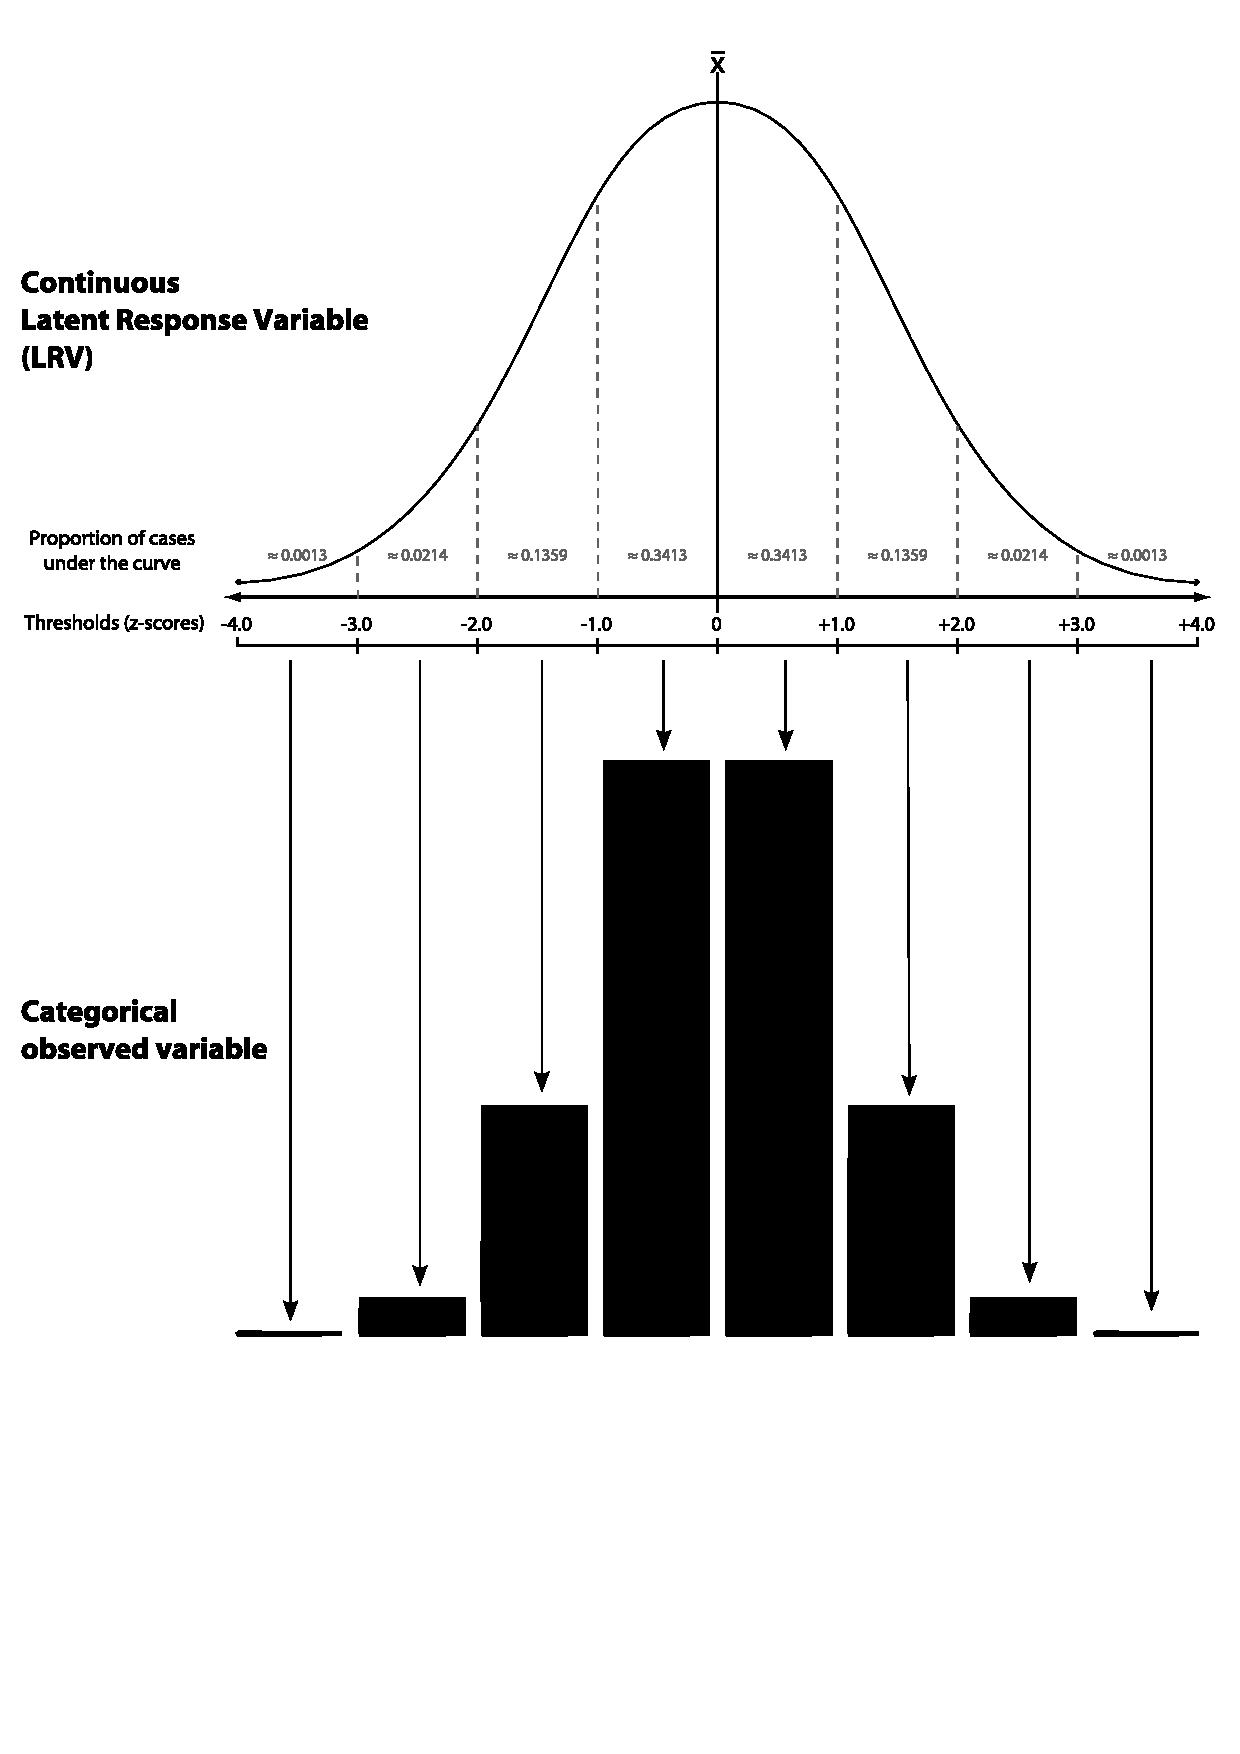
\includegraphics[width=4.5cm]{i/LRV-8cat.pdf}\end{column}
 	\begin{column}<3->{4.5cm} \textbf{country B}

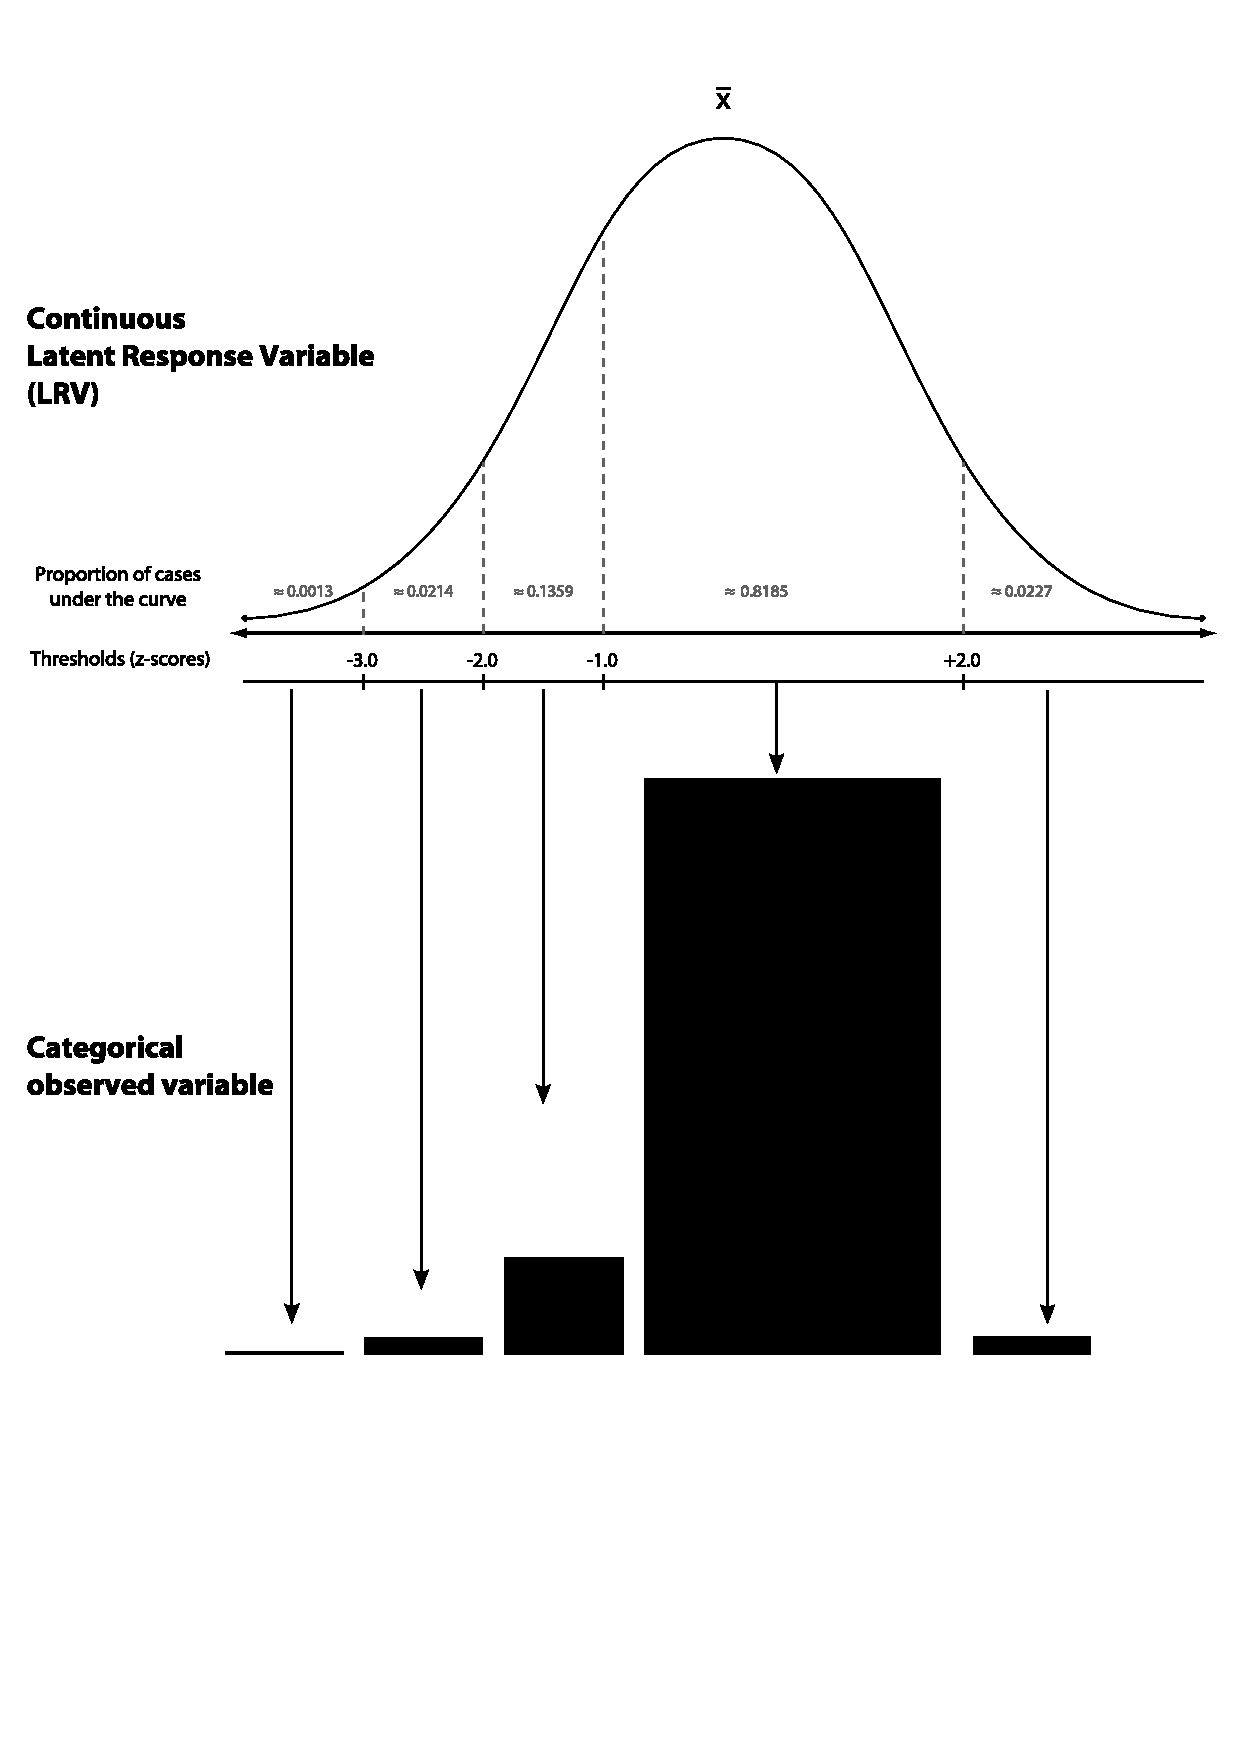
\includegraphics[width=4.5cm]{i/LRV-skew.pdf}
 	\end{column}
 \end{columns}
\end{frame}

\begin{frame}
   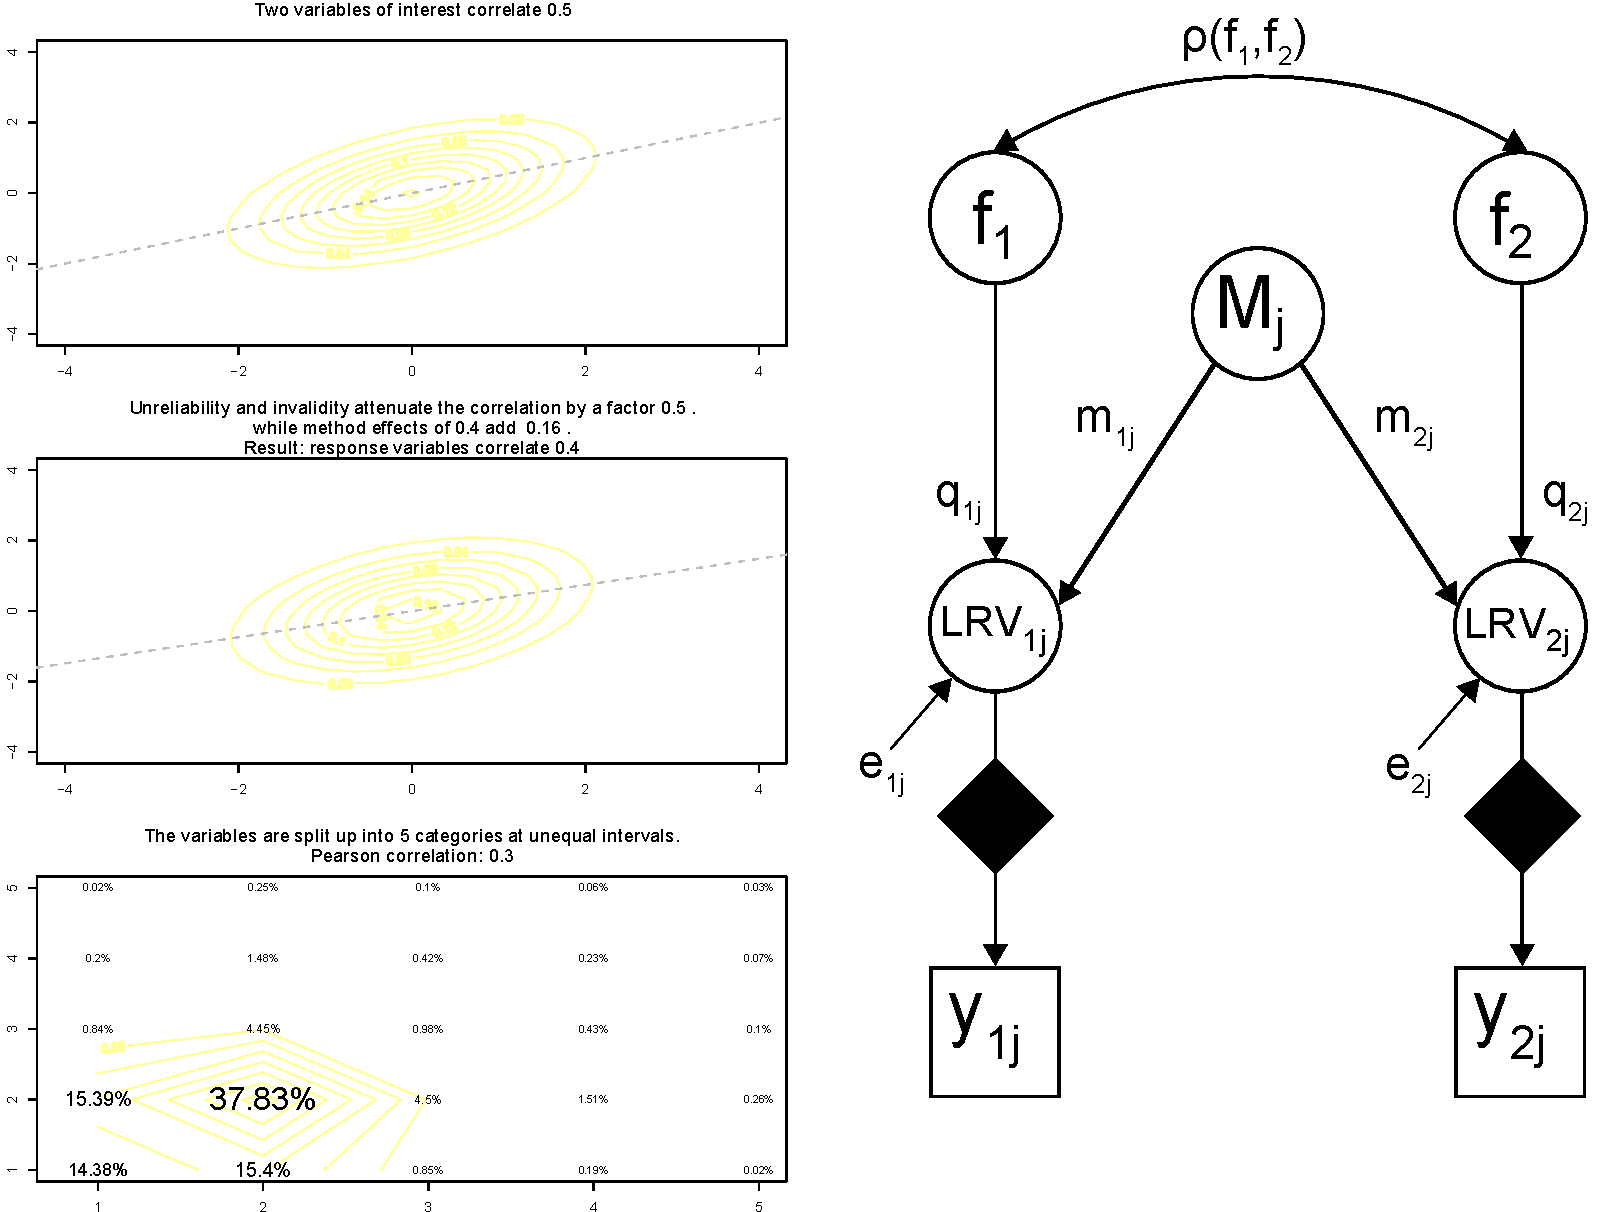
\includegraphics[height=8cm]{i/3_steps_together.pdf}
\end{frame}

\begin{frame}
\frametitle{Two countries with equal qualities but different means}
\begin{columns}<2->[T]
 	\begin{column}{5cm} 
	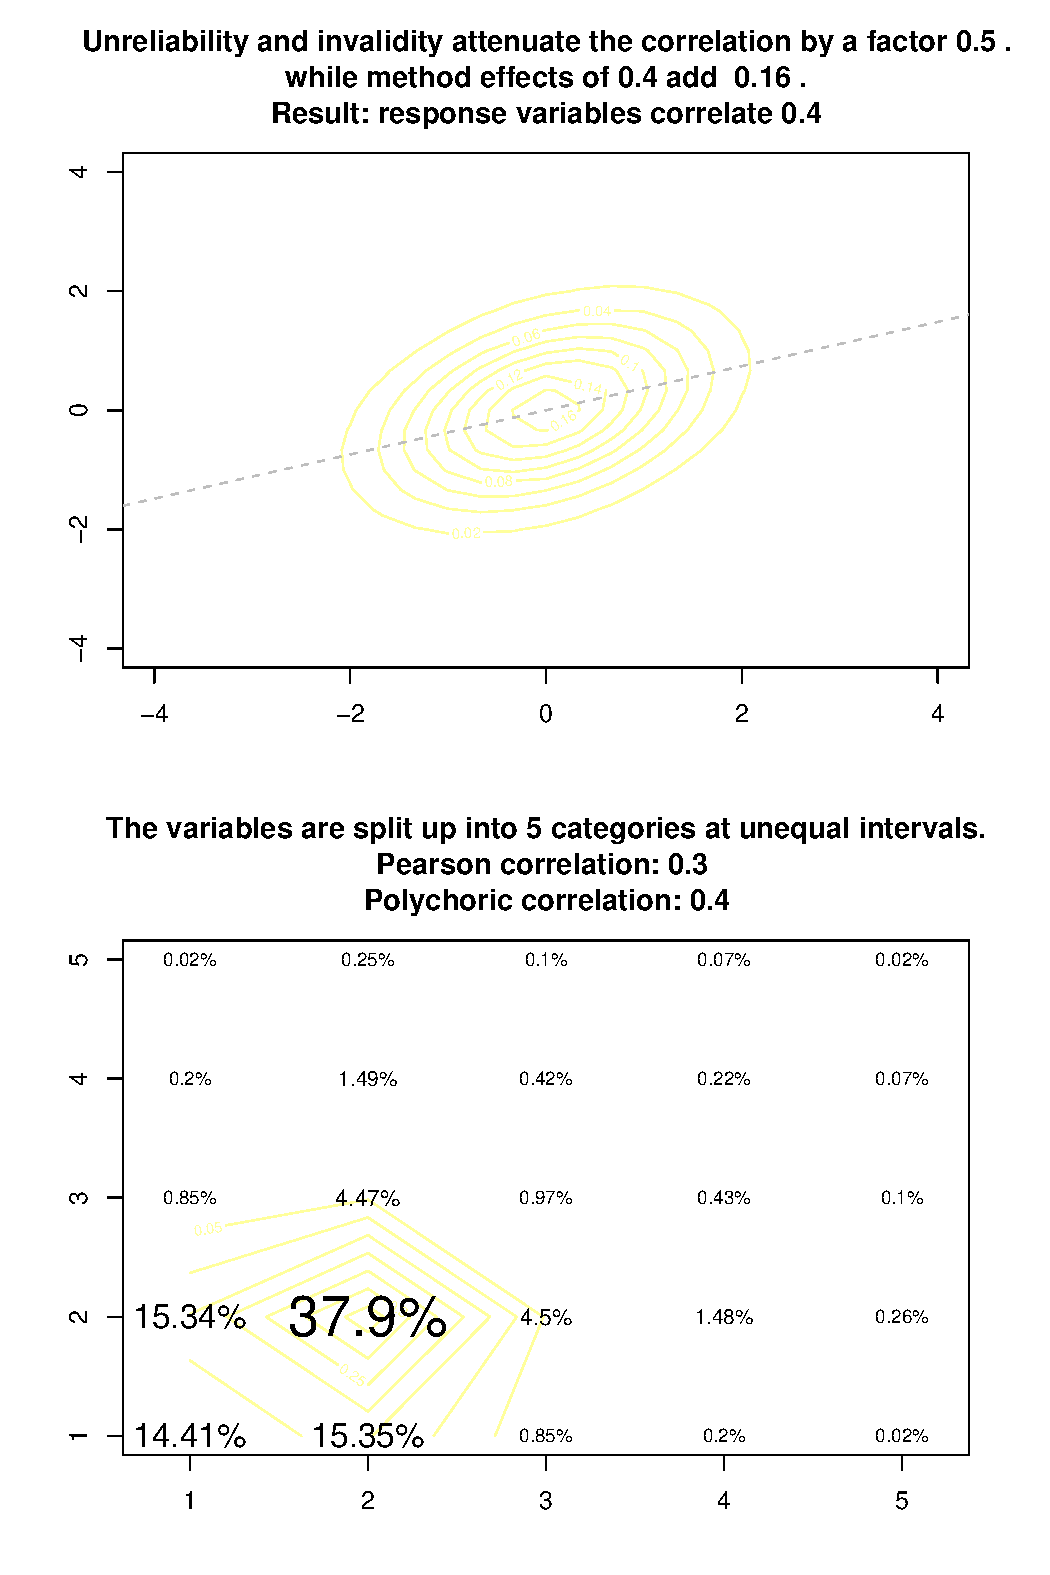
\includegraphics[width=5cm]{i/country_A.pdf}\end{column}
 	\begin{column}<3->{5cm} 
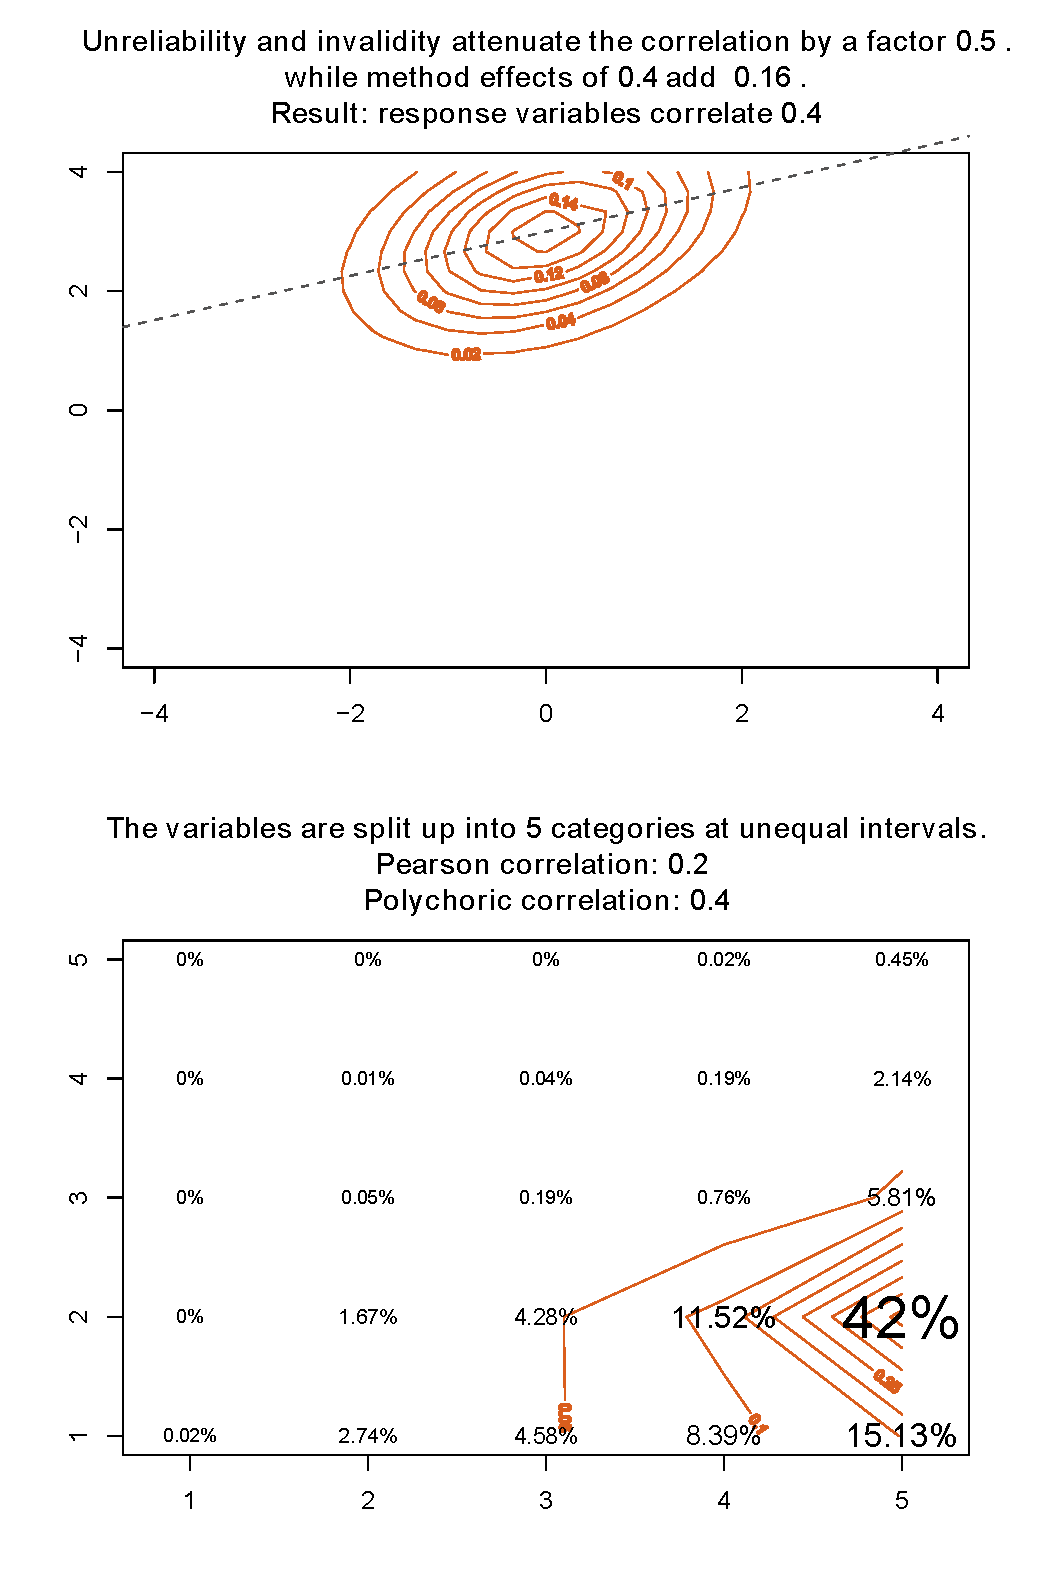
\includegraphics[width=5cm]{i/country_B.pdf}
 	\end{column}
 \end{columns}
\end{frame}


\begin{frame}	
	\frametitle{Categorical data in cross-country studies}
	\begin{itemize}[<alert@+>]
		\item The thresholds used earlier are taken from the estimates of a real experiment!
		\item If the thresholds are different, the observed means and (Pearson) correlations will differ also;
		\item Even a difference in \emph{means} across countries can cause an observed difference in Pearson correlations;
		\item If the assumption of normality holds true, the categorical response model (using polychoric correlations) corrects the LRV correlations;
		\item Whether this model is realistic is the topic of our other presentation.
	\end{itemize}
\end{frame}	

\begin{frame}
	\frametitle{The `categorisation factor'}
	\begin{itemize}
\item The quality was defined as:
		\item \begin{equation*}
q^2 = \frac{Var(f)}{Var(y)}.\label{eqn:relratio}
\end{equation*}
\item However, we have seen that $y$ is itself a categorization of an unobserved continuous variable ($LRV$), and therefore the above equation can be `decomposed' into
\item \begin{equation*}
q^2 =  \frac{ Var(f)}{Var(LRV)} \cdot \frac{Var(LRV)}{Var(y)}.		
\end{equation*}
	\item We call this ratio of the quality coefficient $q = v.r$ from the categorical model to the same coefficient from the continuous model the `categorisation factor'.
	\end{itemize}
\end{frame}

\begin{frame}
	\frametitle{The `categorisation factor'}

	\begin{equation}
	q^2 =  \frac{ Var(f)}{Var(LRV)} \cdot \frac{Var(LRV)}{Var(y)}.		
	\end{equation}

	\begin{itemize}
		\item It can be seen that the quality normally estimated from the continuous model is a product of two terms:
		\item $$
			q^2_{cont} = q^2_{categ} \cdot c,
		$$
		where $c$ is a categorisation factor.
		\item If $c < 1$, the quality in the categorical model is higher than in the continuous model
		\item If $c > 1$, the quality in the categorical model is lower than in the continuous model
	\end{itemize}
\end{frame}

\section{Multitrait-multimethod experiments}
\begin{frame}

\textbf{\centering How can the quality and thresholds be estimated in different countries?}

\end{frame}

\subsection{An example experiment}
\begin{frame}
	\frametitle{First trait measured with three methods}
	\begin{tabular}{l}
		\hline
		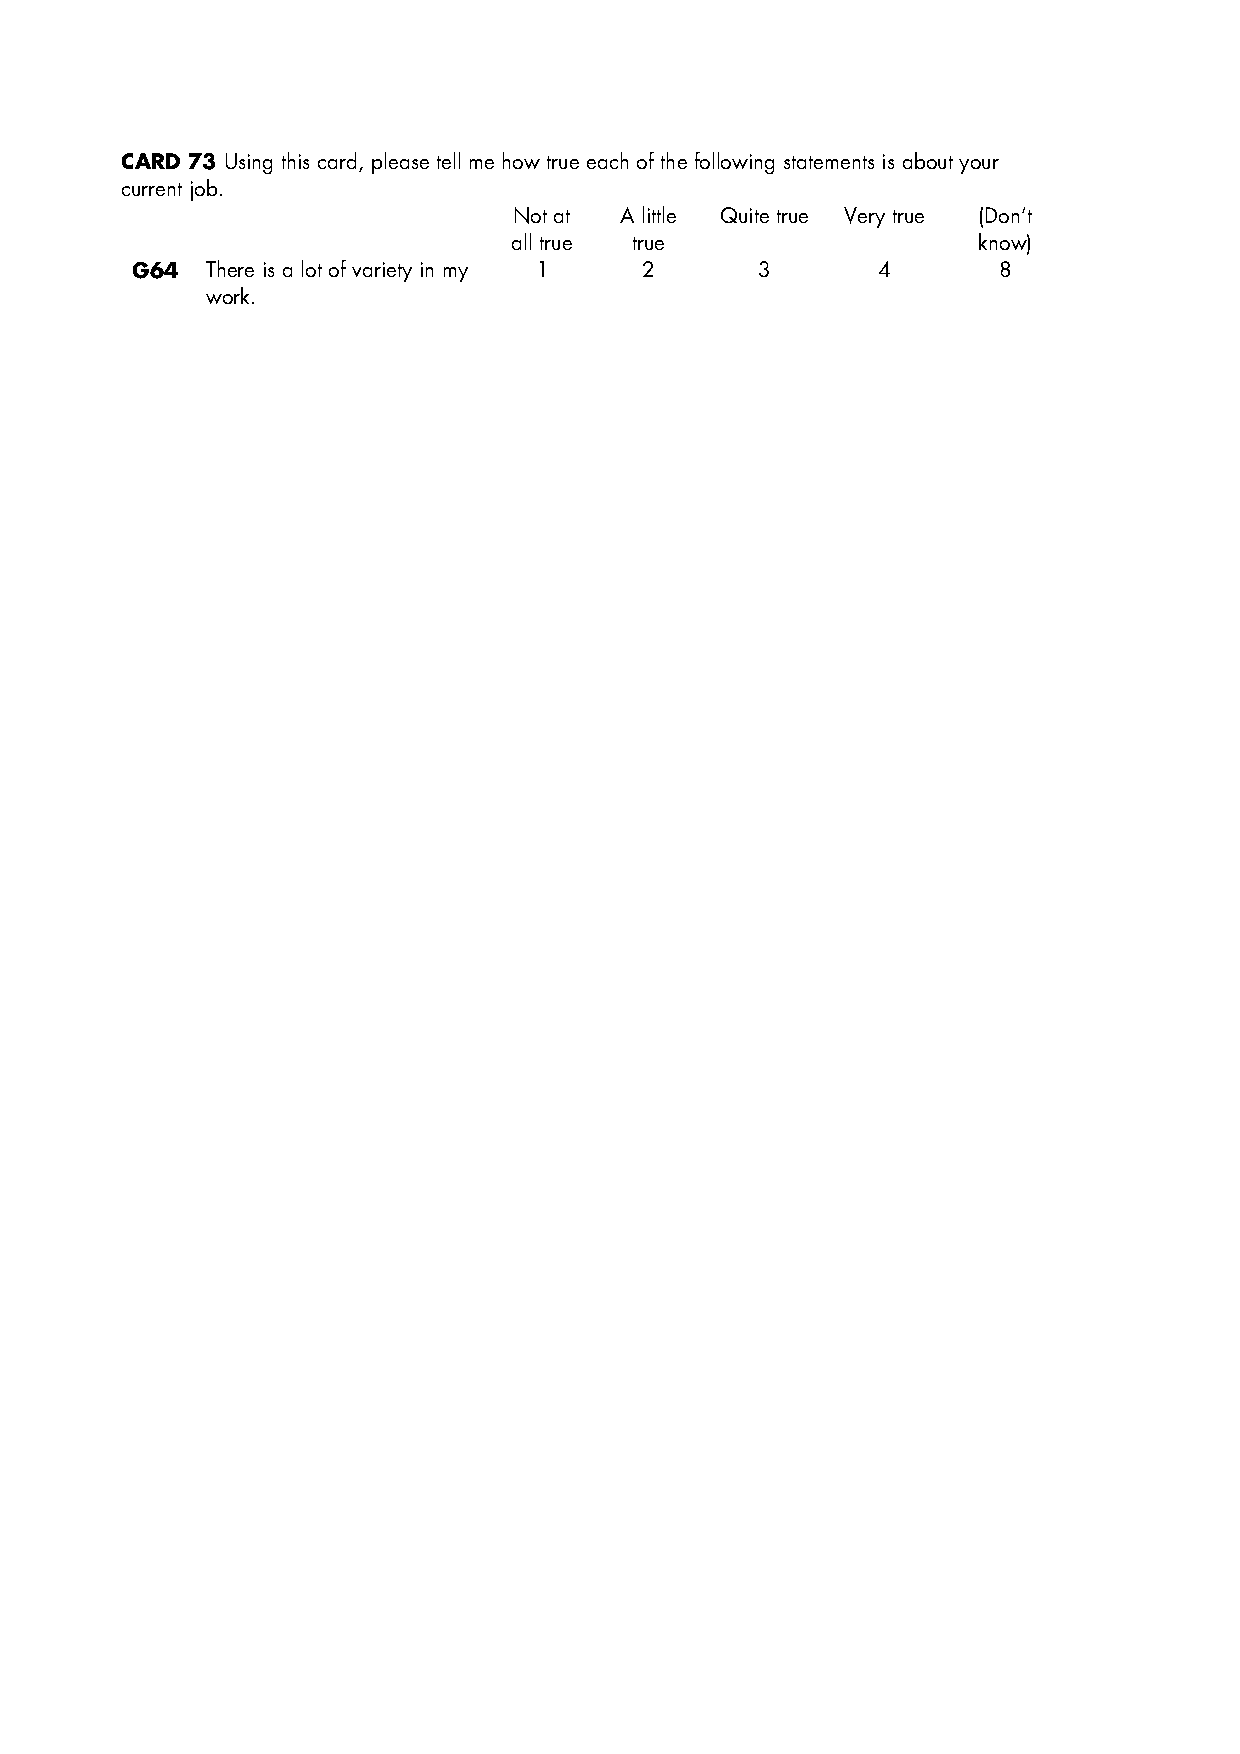
\includegraphics[width=8cm]{i/trait-1-m-1.pdf} \\\hline
		
\includegraphics[width=8cm]{i/trait-1-m-2.pdf} \\\hline
		 
\includegraphics[width=8cm]{i/trait-1-m-3.pdf}\\
		\hline
	\end{tabular}
\end{frame}

\begin{frame}
	\frametitle{Three traits measured with first method}
		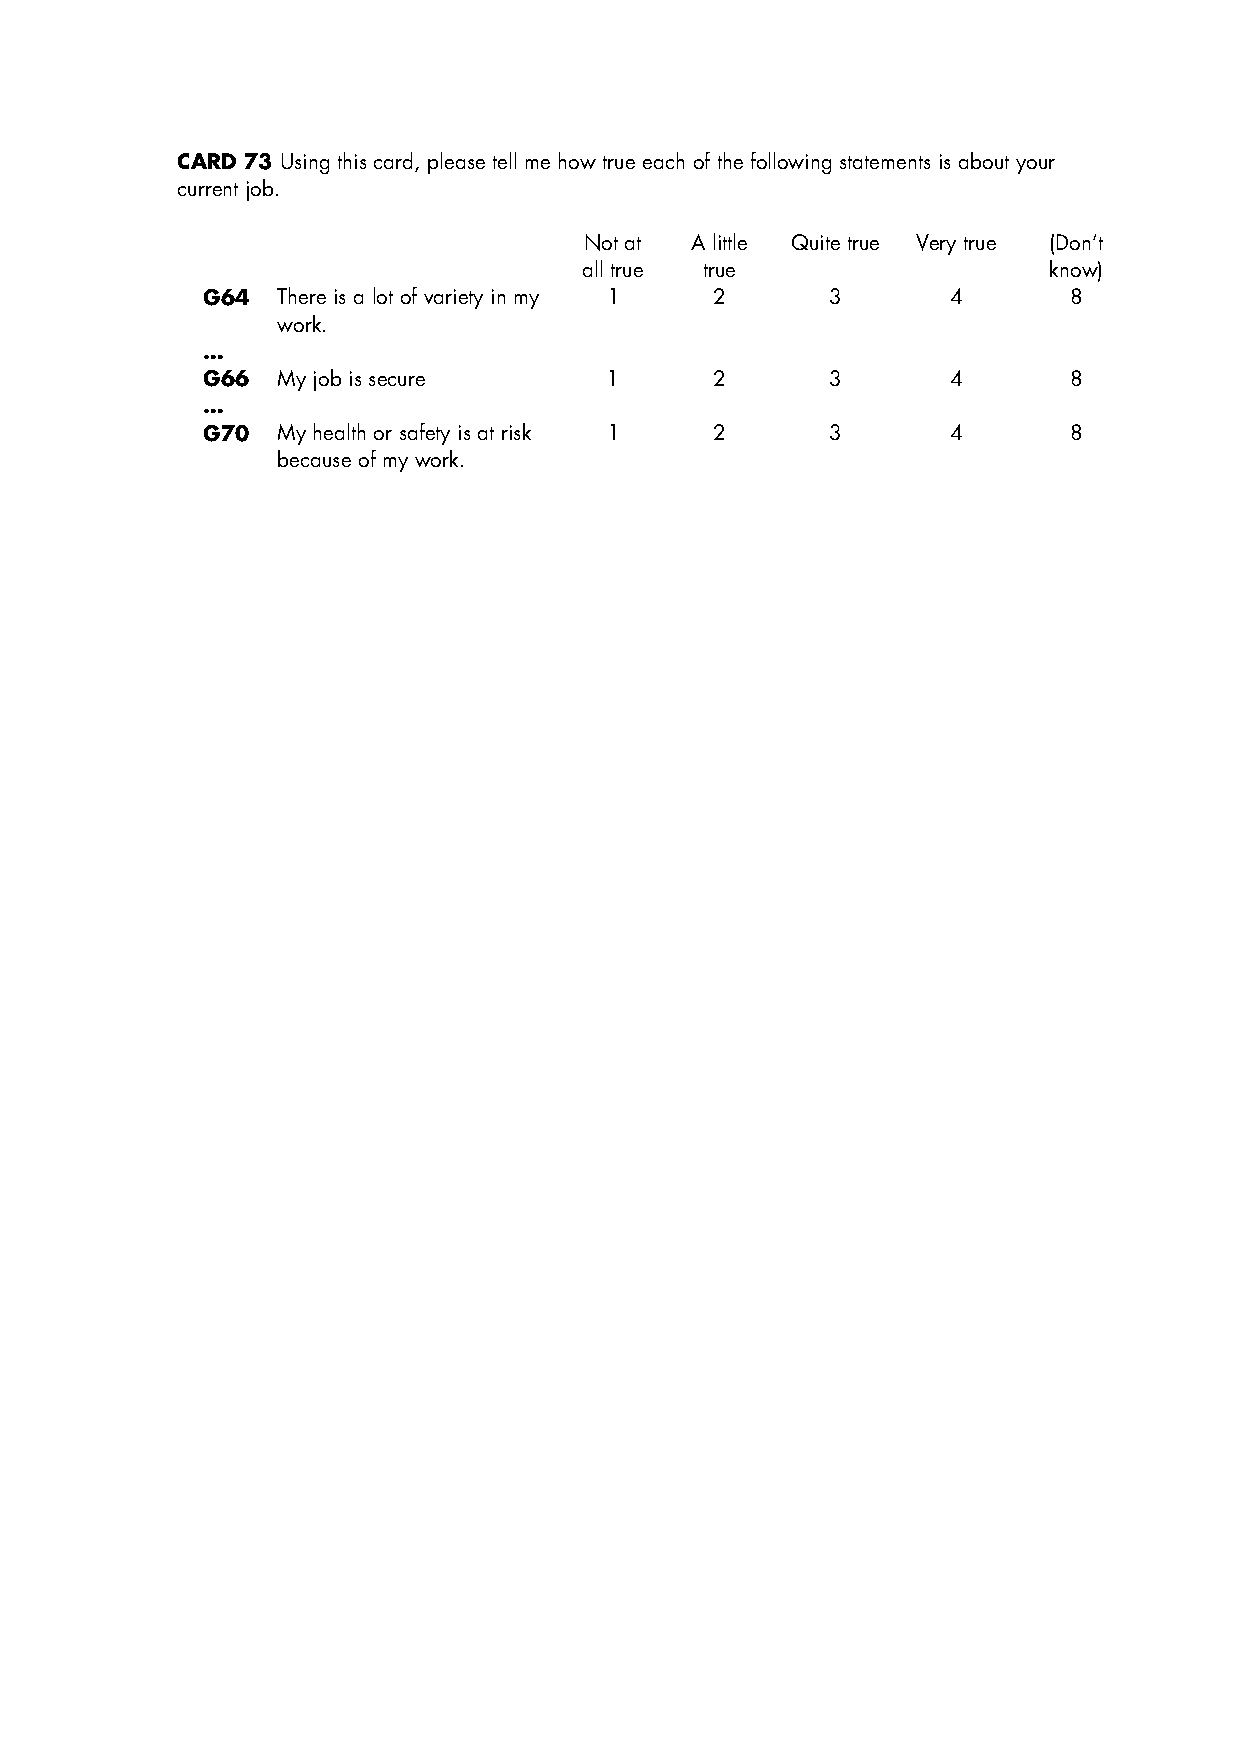
\includegraphics[width=11.2cm]{i/method-1.pdf}
\end{frame}

\begin{frame}
	\frametitle{Three traits measured with second method}
		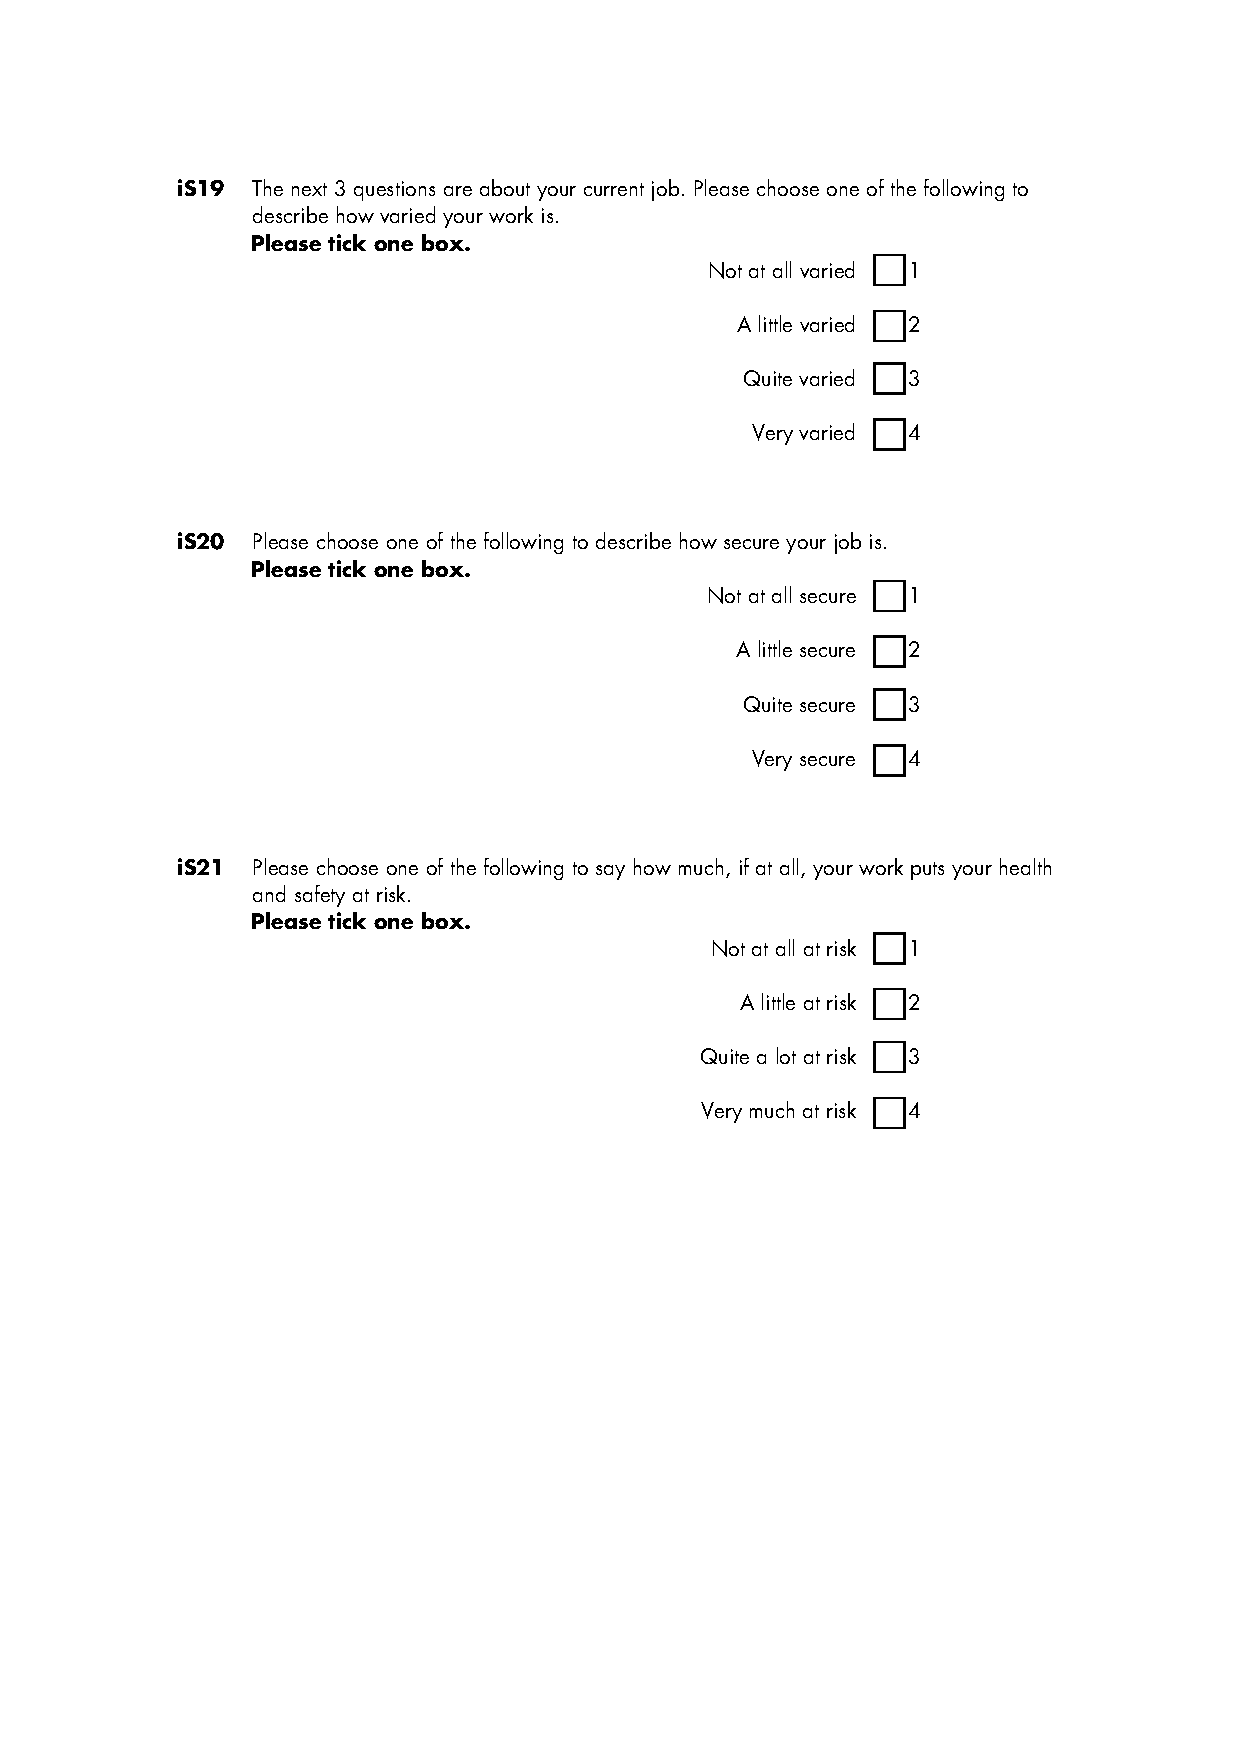
\includegraphics[height=7cm]{i/method-2.pdf}
\end{frame}

\begin{frame}
	\frametitle{Three traits measured with third method}
	\begin{columns}[T]
		\begin{column}{7cm}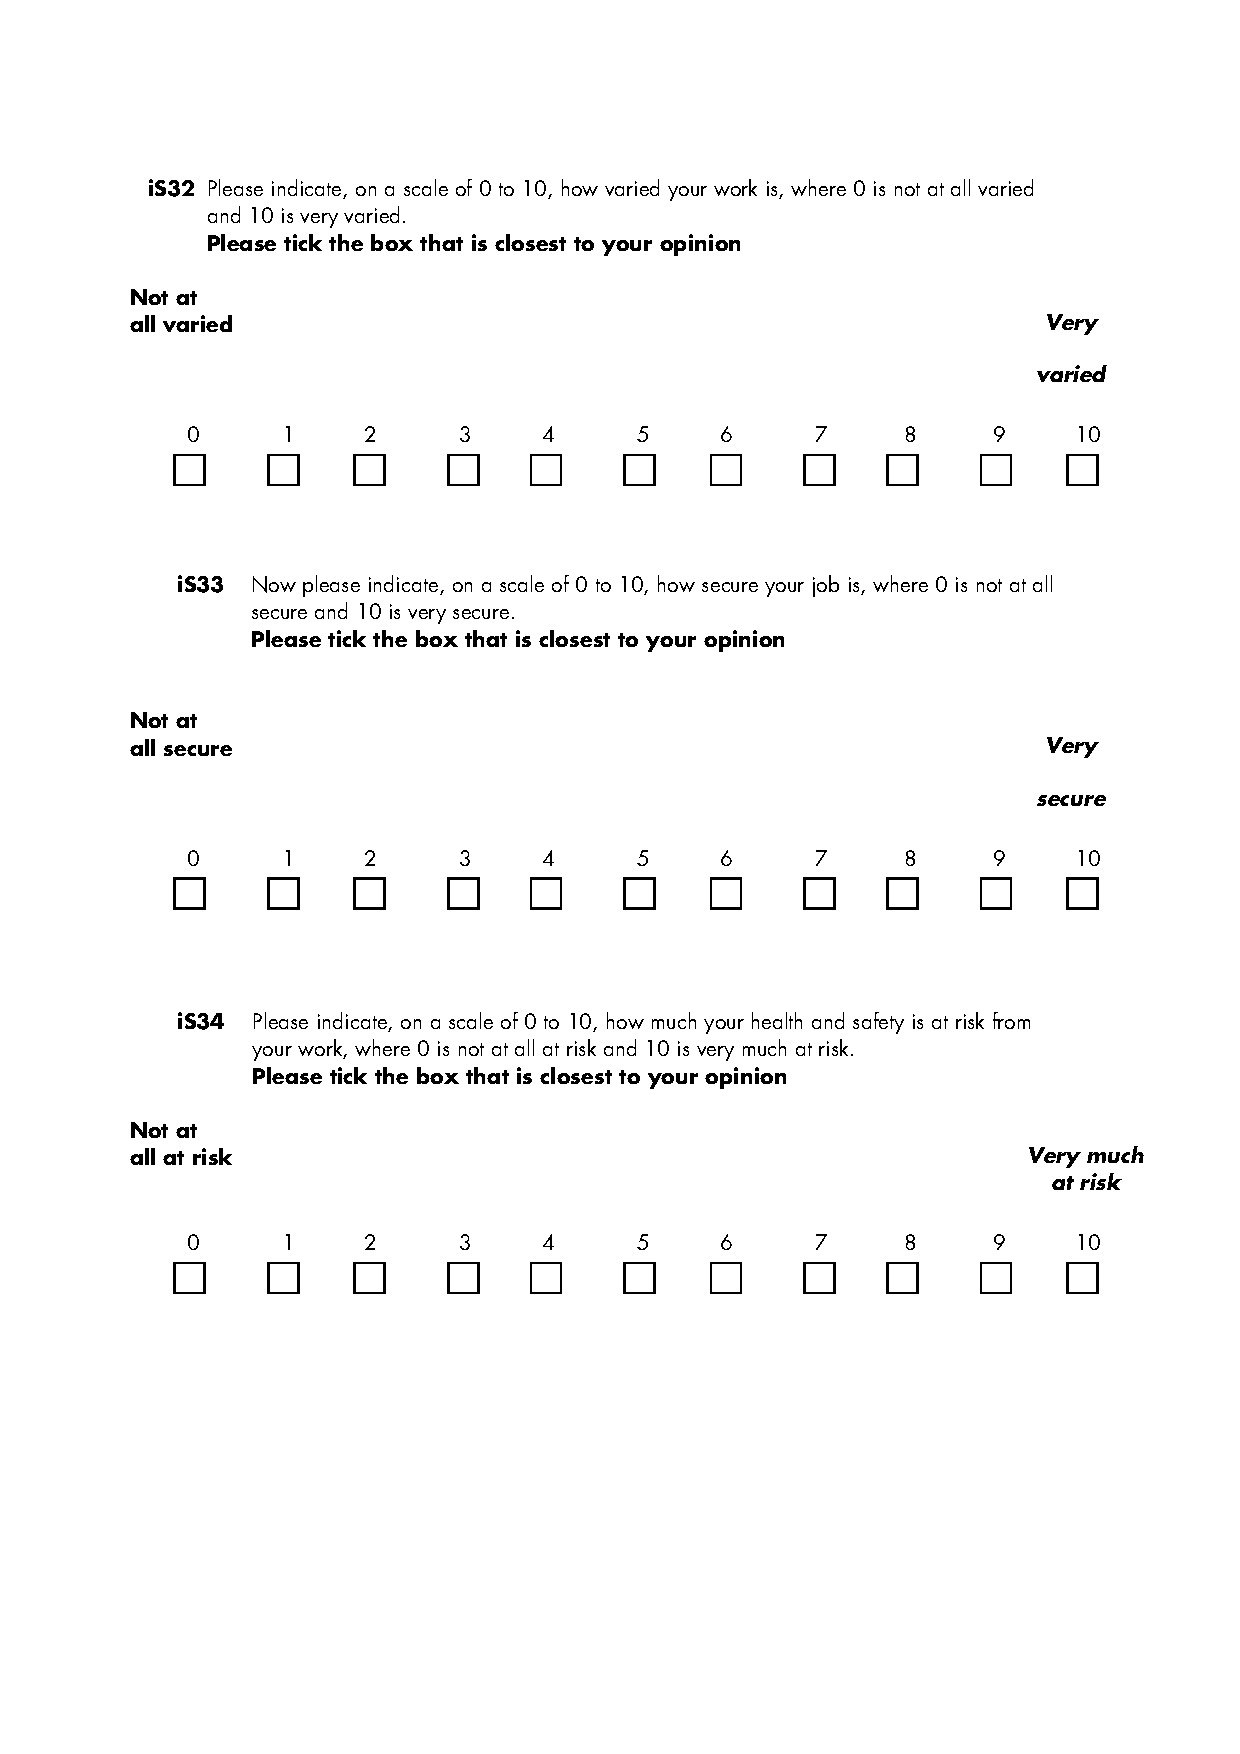
\includegraphics[height=7cm]{i/method-3.pdf}\end{column}
		\begin{column}{3cm}\hyperlink{model}{\beamerbutton{Skip details of the model}}\end{column}
	\end{columns}		
\end{frame}

\if 1=2
\subsection{Designs}

\begin{frame}	
	\frametitle{Split ballot design}

	\begin{itemize}[<alert@+>]
		\item Different designs are possible
		\item If 3 traits are asked using 3 methods, the respondent has to answer 
			$3 \times 3 = 9$ questions per experiment
		\item Answering the same question 3 times, for three different questions is a large response burden
		\item The solution: split ballot MTMM design.
\item<5-|alert@5> {
	Split the sample into groups A and B:

	\begin{tabular}{llccc}
\hline
		&&\multicolumn{3}{c}{Trait}\\
		& Method & 1 & 2 & 3\\
\hline
		Main quest. 	& 1 & A,B & A,B & A,B\\
		Supplementary quest.	& 2 & A & A & A\\
							& 3 & B & B & B\\
\hline
	\end{tabular}	}
	\end{itemize}

\end{frame}	
\fi

\subsection{Models}

\begin{frame}	
	\frametitle{Different models for MTMM experiments}
	\begin{itemize}[<alert@+>]
		\item Classic MTMM model
		\item Correlated uniqueness (Kenny \& Judd)
		\item Direct product (Browne)
		\item True score model
		\item MTM-1 (Eid 2000)
	\end{itemize}
\end{frame}	
\begin{frame}	
	\frametitle{Different models for MTMM experiments}
	\begin{itemize}[<alert@+>]
		\item We use the true score model
		\item Equivalent to the classic MTMM model
		\item Sometimes necessary to remove one method factor
		\item In that case our model is the equivalent to Eid's MTM-1 model.
	\end{itemize}
\end{frame}	

\begin{frame}	
	\frametitle{\hypertarget{model}{True score model}}
	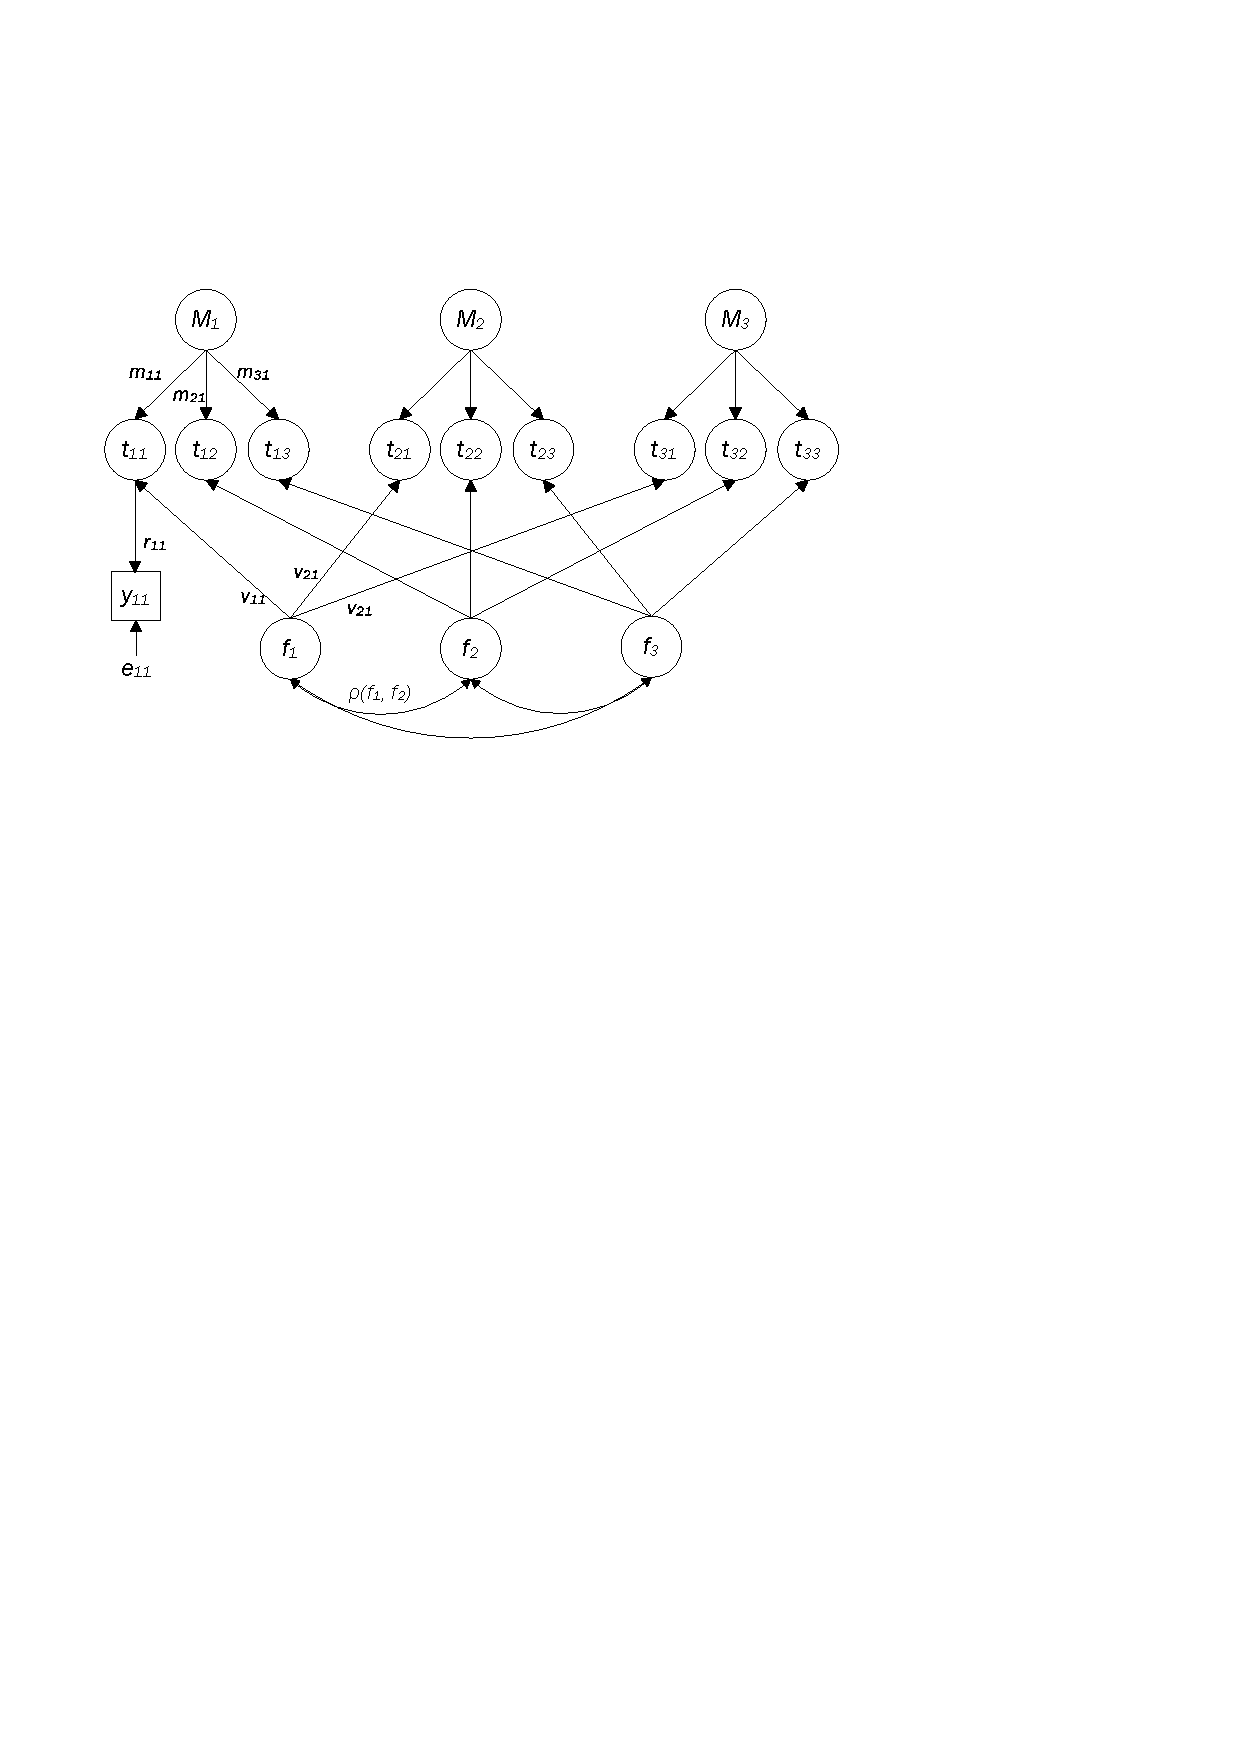
\includegraphics[height=7cm]{i/MTMM.pdf}
	\framezoom<1><2>(0cm,1.85cm)(.5cm,4.5cm)
	\framezoom<1><3>(0cm,0cm)(1cm,3cm)
\end{frame}	

\begin{frame}	
	\frametitle{True score model assumptions}
	\begin{itemize}[<alert@+>]
		\item No correlations among methods
		\item No correlations between traits and methods
		\item Equal method effects
		\item Linear and additive effects
		\item Normal errors, independent of all unobserved variables
		\item All variables are continuous
	\end{itemize}
\end{frame}	



\if 1=2
\begin{frame}
    \begin{itemize}
    \item These continuous latent response variables are related to each other according to the MTMM model.
	\item Method effects, quality coefficients, and thresholds can be estimated.
    \item Equivalent to a 2 parameter graded response model in IRT (Muth\'en \& Asparouhov 2002).
    \end{itemize}
\end{frame}
\fi

\begin{frame}
\frametitle{Consequences of categorisation for the correlations between observed variables}

	\begin{itemize}[<alert@+>]
		\item The fewer categories, the smaller the Pearson correlation;
		\item The more skew in observed variables, the smaller the Pearson correlation;
		\item The corrected (`polychoric') correlations are generally higher than the Pearson correlations, but not necessarily equally so for all variables.
	\end{itemize}
\end{frame}

\begin{frame} 
	Therefore,
	\begin{itemize}[<alert@+>]
		\item If the skewness of observed variables is higher for variables measured by one particular method, then the corrected correlations between those variables will go up more than the others, and the method effects in the categorical model will be higher;
		\item As method-induced correlation goes up, the estimates of the quality will go down instead of up!
	\end{itemize} 
\end{frame}

\begin{frame}
\frametitle{Analysis of the experiments}

	\begin{itemize}[<alert@+>]
		\item We analysed the 4 experiments from the ESS which involved variables with 5 categories or less
		\item The topics: role of women, GP's, political efficacy, job.

			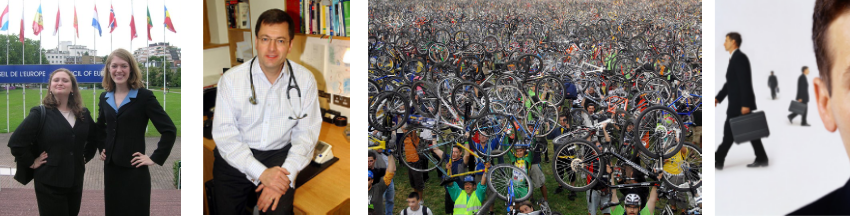
\includegraphics[width=10cm]{i/topics.png} 

	\item Compare the country with the highest quality to the country with the lowest quality for that experiment (not discussed here)
	\end{itemize}
\end{frame}


\subsection{Categorisation errors in the efficacy experiment}

\begin{frame}
\frametitle{Quality ($q^2$)and method effects ($m$) in the efficacy experiment, in Denmark}

Results of continuous MTMM model, main questionnaire (first method)

\begin{footnotesize}\begin{tabular}{llrrr}
\hline
 &  &  &   `Efficacy' & \\
&  &   Complex & Active & Mind\\
	   \hline
 &  $q^2$&   0.77 & 0.83 & 0.79\\
 &  $m$&   0.00 & 0.00 & 0.00\\
\hline
\end{tabular}


$df=19, \chi^2=40.0, p = 0.003$.
\end{footnotesize}
\end{frame}


\begin{frame}
\frametitle{Efficacy experiment: Denmark}
\begin{footnotesize}
Polychoric correlations
\begin{tabular}{llrrrrrr}
 \hline
 &&\multicolumn{3}{c}{Method 1} & \multicolumn{3}{c}{Method 2}\\
 &&\multicolumn{3}{c}{$\overbrace{\hspace{90pt}}$} & \multicolumn{3}{c}{$\overbrace{\hspace{90pt}}$}\\
Method 1	& Complex 	& 1.00 \\
			& Active 	& -0.44 & 1.00 \\
			& Mind 		& -0.51 & 0.47 & 1.00 \\
Method 2	& Complex 	& 0.66 & -0.45 & -0.51 & 1.00 \\
			& Active 	& -0.44 & 0.74 & 0.46 & -0.51 & 1.00  \\
			& Mind 		& -0.52 & 0.51 & 0.67 & -0.56 & 0.56 & 1.00\\
 \hline
 \end{tabular}

Pearson correlations

\begin{tabular}{llrrrrrr}
 \hline
 &&\multicolumn{3}{c}{Method 1} & \multicolumn{3}{c}{Method 2}\\

 &&\multicolumn{3}{c}{$\overbrace{\hspace{90pt}}$} & \multicolumn{3}{c}{$\overbrace{\hspace{90pt}}$}\\
Method 1	& Complex 	& 1.00\\
			& Active 	&-0.38 & 1.00\\
			& Mind 		&-0.46 & 0.41 & 1.00\\
Method 2	& Complex 	& 0.60 & -0.37 & -0.44 & 1.00\\
			& Active 	&-0.39 & 0.67 & 0.40 & -0.43 & 1.00\\
			& Mind 		&-0.46 & 0.43 & 0.62 & -0.49 & 0.48 & 1.00\\
 \hline
 \end{tabular} 

$n \approx 916$
\end{footnotesize}

\end{frame}


\if 1=2
\begin{frame}
\frametitle{Efficacy experiment: Switzerland}
\begin{footnotesize}

Polychoric correlations

\begin{tabular}{llrrrrrr}
 \hline
 &&\multicolumn{3}{c}{Method 1} & \multicolumn{3}{c}{Method 2}\\
 &&\multicolumn{3}{c}{$\overbrace{\hspace{90pt}}$} & \multicolumn{3}{c}{$\overbrace{\hspace{90pt}}$}\\
Method 1	& Complex 	& 1.00 & \\
			& Active 	& -0.37 & 1.00 & \\
			& Mind 		& -0.46 & 0.42 & 1.00 & \\
Method 2	& Complex 	& 0.57 & -0.36 & -0.46 & 1.00 & \\
			& Active 	& -0.32 & 0.83 & 0.36 & -0.39 & 1.00 & \\
			& Mind 		& -0.36 & 0.44 & 0.69 & -0.49 & 0.43 & 1.00\\
 \hline
 \end{tabular} 

Pearson correlations

\begin{tabular}{llrrrrrr}
 \hline
 &&\multicolumn{3}{c}{Method 1} & \multicolumn{3}{c}{Method 2}\\
 &&\multicolumn{3}{c}{$\overbrace{\hspace{90pt}}$} & \multicolumn{3}{c}{$\overbrace{\hspace{90pt}}$}\\
Method 1	& Complex 	&  1.00\\
			& Active 	& -0.33 & 1.00\\
			& Mind 		& -0.43 & 0.36 & 1.00\\
Method 2	& Complex 	&  0.55 & -0.35 & -0.45 & 1.00\\
			& Active 	& -0.30 & 0.82 & 0.33 & -0.34 & 1.00\\
			& Mind 		& -0.35 & 0.41 & 0.62 & -0.48 & 0.39 & 1.00\\
 \hline
 \end{tabular} 

$n \approx 779$
\end{footnotesize}
\end{frame}\fi

\begin{frame}
\frametitle{\% Increase in the correlations after correction for categorisation}

Efficacy experiment: Denmark

\begin{tabular}{llrrrrrr}
\hline
 &&\multicolumn{3}{c}{Method 1} & \multicolumn{2}{c}{Method 2}  \\
&&\multicolumn{3}{c}{$\overbrace{\hspace{90pt}}$} & \multicolumn{3}{c}{$\overbrace{\hspace{60pt}}$}\\
Method 1	& Complex 	& \\
			& Active 	& \textbf{16}\%\\
			& Mind 		& \textbf{11}\% & \textbf{15}\%\\
Method 2	& Complex 	& 10\% & 22\% & 16\%\\
			& Active 	& 13\% & 10\% & 15\% & \textbf{19}\%\\
			& Mind 		& 13\% & 19\% & 8\% &  \textbf{14}\% & \textbf{17}\%\\
\hline
\end{tabular}

Mean percentage increase of the polychoric correlations:  14.5\%

%> approx.power(2.187, 79.889, alpha=.05)
%[1] 0.05
\end{frame}



\if 1=2
\begin{frame}
\frametitle{\% Increase in the correlations after correction for categorisation}

Efficacy experiment: Switzerland

\begin{tabular}{llrrrrrr}
\hline
 &&\multicolumn{3}{c}{Method 1} & \multicolumn{2}{c}{Method 2}  \\
&&\multicolumn{3}{c}{$\overbrace{\hspace{90pt}}$} & \multicolumn{3}{c}{$\overbrace{\hspace{60pt}}$}\\
Method 1	& Complex 	&    &  &  &  &  & \\
			& Active 	& \textbf{12}\% &  &  &  &  & \\
			& Mind 		&   \textbf{8}\% & \textbf{17}\% &  &  &  & \\
Method 2	& Complex 	&   4\% & 3\% & 3\% &  &  & \\
			& Active 	&   6\% & 1\% & 1\% & \textbf{16}\% &  & \\
			& Mind 		&   2\% & 7\% & 12\% & \textbf{3}\% & \textbf{1}\% & \\
\hline
\end{tabular}

Mean percentage increase of the polychoric correlations: 7.6\%
\end{frame}

\begin{frame}
\frametitle{Consequences of correction for categorisation}
	\begin{itemize}[<alert@+>]
		\item In both Denmark and Switzerland, the monomethod correlations increase more than the other correlations;
		\item In the continuous analysis, no significant method factor was found for the first method in either country;
		\item In \textbf{Denmark} the monomethod correlations were already relatively high, however, leading to a significant method factor in the categorical model;
		\item This leads to a lower quality estimate than in the continuous model in Denmark.
		\item In \textbf{Switzerland} the monomethod correlations were lower; 
		\item No significant method factor is found there, and the `upwards push' can therefore increase the quality coefficients.
	\end{itemize}
\end{frame}

\fi


\begin{frame}
\frametitle{Quality ($q^2$)and method effects ($m$) according to the continuous and categorical models, with categorisation factors}

\begin{footnotesize}\begin{tabular}{llrrr}
\hline
 &  &  &   `Efficacy' & \\
	   &  &   Complex & Active & Mind\\
	   \hline
 \multicolumn{2}{l}{Continuous analysis}\\
 &  $q^2$&  0.77 & 0.83 & 0.79  \\
 &  $m$&  0.00 & 0.00 & 0.00\\
\multicolumn{4}{l}{Categorical analysis} \\
 &  $q^2$&  0.63 & 0.70 & 0.63  \\
 &  $m$&  0.11 & 0.08 & 0.11 \\
\multicolumn{2}{l}{Categorisation factor}      &  & \\
 &  &  1.23 & 1.18 & 1.25 \\
\hline
\end{tabular}

\end{footnotesize}
\end{frame}


\begin{frame}
\frametitle{Correction for categorisation: conclusions}

\begin{itemize}[<alert@+>]
   \item The general `push'  is that all coefficients go up, because the polychoric correlations are always higher than the Pearson correlations;
   \item But when method factors are taken into account, the coefficients can also go down;
   \item This happens especially when the method variance is estimated at zero in the continuous model, but cannot be so constrained in the categorical model.
	\item Would then expect countries with high quality to have a lower quality after correction for categorisation and vice versa.
	\end{itemize}
\end{frame}

\section{A meta-analysis of the categorisation error studies}
\begin{frame}\begin{center}
The categorisation factor, $q_{cat}/q_{cont}$:
 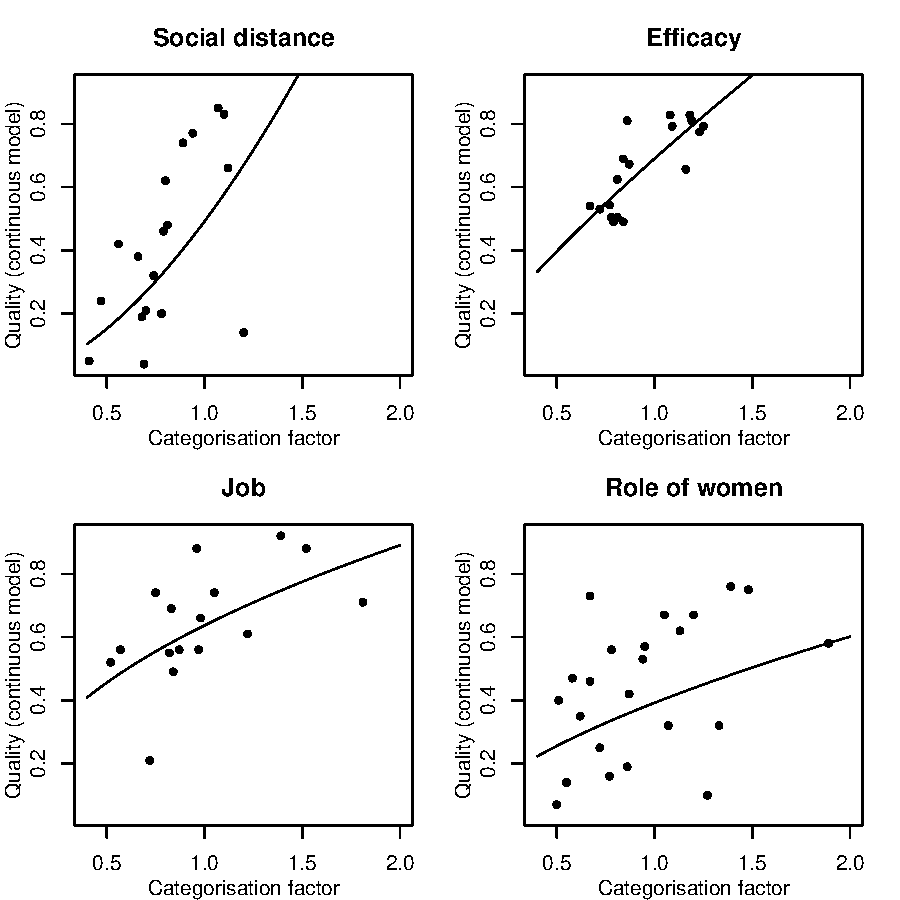
\includegraphics[height=7.4cm]{../latex/i/predict_q2.pdf} 
\end{center}
\end{frame}

\begin{frame}
\frametitle{How general are the findings?}

\begin{footnotesize}

\begin{tabular}{llrrrr}
\hline
& & & & \multicolumn{2}{c}{95\% C.I}\\
 &  & Estimate & S.E. & lower & upper\\
 \hline
&(Intercept) & 1.04 & 0.36 & 0.31 & 1.77 \\ 
\multicolumn{2}{l}{\textit{Topic}}&  &  &  & \\
 & Doctors & (reference category) &  &  & \\
&Efficacy & 0.06 & 0.10 & -0.14 & 0.27 \\ 
&Job & 0.04 & 0.40 & -0.71 & 0.78 \\ 
&Women & 0.38 & 0.26 & -0.14 & 0.90 \\ 
\multicolumn{2}{l}{\textit{Scale}}&  &  &  & \\ 
 & Direct  & (reference category) &  &  & \\
&Agree-disagree & -0.11 & 0.35 & -0.81 & 0.59 \\ 
&True-false & 0.17 & 0.32 & -0.48 & 0.81 \\ 
\multicolumn{2}{l}{\textit{}   }&  &  &  & \\
\multicolumn{2}{l}{Negative} & -0.50 & 0.23 & -0.96 & -0.02 \\ 
\multicolumn{2}{l}{Main questionnaire} & -0.30 & 0.29 & -0.88 & 0.29 \\ 
\multicolumn{2}{l}{Highest quality} & -0.19 & 0.09 & -0.37 & -0.01 \\ 
\multicolumn{2}{l}{Highest quality $\times$ main} & 0.66 & 0.15 & 0.35 & 0.96 \\ 
\hline
\end{tabular}
Multiple R-Squared: 0.45; Adjusted R-squared: 0.35 

\end{footnotesize}
\end{frame}


\begin{frame}
\frametitle{Some implications of the findings}

\begin{itemize}
   \item Potentially, if one method produces more categorisation errors than another, the quality coefficients may be estimated higher in the continuous model.
   \item If this happens more in some countries than others, differences in quality will result due to the way the LRV's have been categorised.
\end{itemize}
\end{frame}

\begin{frame}
\frametitle{The latent traits}

Estimated correlations between the latent traits under the two different models

\begin{tabular}{lrrr}
\hline
	 & Complex & Active & Mind\\
\hline
Continuous model & 1\\
&-.63  &     1\\
&-.75   &    .66   &   1\\
&\\
Categorical model &1 \\
&-.63 & 1\\
&-.75  & .70 & 1\\
\hline
\end{tabular}
\end{frame}

\section{Conclusion}

\begin{frame}

\frametitle{Conclusions}
\begin{itemize}[<alert@+>]
   \item It was possible to split the measurement error model into three parts:
      \begin{itemize}
	 \item A part due to random errors;
	 \item A part due to systematic errors;
	 \item A part due to splitting the variable into just a few categories.
      \end{itemize}
   \item The estimates one gets can differ, and not always in the way one might expect;
   \item The correlations between the latent traits corrected for measurement error in this experiment were robust to the model specification;
   \item This suggests either model will provide a correct (or at least similar) inference about the variables of interest in this case.
\end{itemize}
\end{frame}


\begin{frame}
\frametitle{Further study, problems}
	\begin{itemize}[<alert@+>]
				\item Investigate normality assumption (tests indicate possible issues), linearity;
				\item Unobserved heterogeneity;
				\item Prediction of the data quality based on characteristics of the question.
			\end{itemize}
\end{frame}

\begin{frame}
That's it for now. Moltes gr�cies per la seva atenci�!

\vspace{1em}\begin{footnotesize}
	\begin{columns}[T]
		\begin{column}{3cm}\centering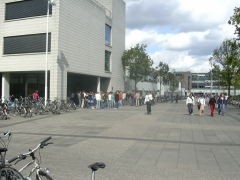
\includegraphics[width=2.55cm]{i/uvt_fac.jpg} 

Tilburg\end{column}
		\begin{column}{3cm}\centering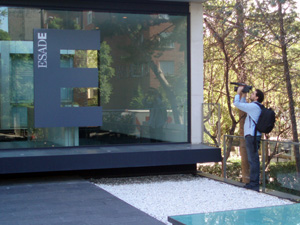
\includegraphics[width=2.5cm]{i/esade_fac.jpg} 

Barcelona\end{column}
	\end{columns}		
\end{footnotesize}
\end{frame}



\section{Epilogue}

\begin{frame}
 \frametitle{The final goal: Survey Quality Predictor (SQP)}

	\begin{enumerate}[<alert@+>]
		\item Estimate the model for all experiments
		\item Save the reliability, validity, and method effect coefficients
		\item Relate the coefficients to different aspects of the question
			\begin{itemize}[<4-|alert@+>]
				\item Complexity of the sentence: no. words/sentence, avg. no. syllables, ...
				\item Response scale: type, no. categories, ...
				\item Formulation of the request: agree-disagree, extra information, ...
				\item Data collection method: computer assisted, interviewer present, ...
			\end{itemize}
		\item Predict the quality of survey questions from their characteristics (SQP)
		\item Improve survey questions
		\item \texttt{http://www.sqp.nl} 
	\end{enumerate}
\end{frame}


\begin{frame}
 \frametitle{References of interest}

\begin{thebibliography}{10}
\bibitem{Saris2008}
Saris, Willem, Albert Satorra, and William van der Veld
\newblock Testing Structural Equation models or Detection of misspecifications? 
\newblock Forthcoming in \emph{Structural Equation Modeling: an interdisciplinary journal}.
\end{thebibliography}

\end{frame}


\end{document}
